\chapter{Oprogramowanie symulacyjne}
\label{ch:simulation-app}

Na potrzeby pracy zostało stworzone oprogramowanie symulacyjne, które posłużyło do przeprowadzenia testów algorytmów planowania oraz wizualizacji ich działania.
W tym rozdziale opisano techniczne rozwiązania wykorzystane podczas tworzenia oprogramowania.
W aplikacji zostały zaimplementowane algorytmy planowania tras opisane w rozdziale \ref{ch:alg-impl}.
Prezentacja ich działania odbywa się poprzez wizualizację ruchu robotów w czasie rzeczywistym. 

\section{Funkcjonalności aplikacji}
Aplikacja umożliwia dowolne definiowanie przez użytkownika środowiska, w którym poruszają się roboty. Obejmuje to:
\begin{itemize}
	\item wybór rozmiaru mapy - dowolną wysokość oraz szerokość. Mapa nie musi być kwadratowa.
	\item możliwość wygenerowania mapy za pomocą generatora labiryntów (por. \ref{ch:mazegen}) lub manualnego umieszczania przeszkód na mapie za pomocą myszki,
	\item wybór liczby robotów i dokonanie ich automatycznego rozmieszczenia na mapie (w losowych polach z pominięciem pól zajętych). Użytkownik ma także możliwość manualnego dodawania i usuwania robotów.
\end{itemize}

Aplikacja przeprowadza symulację ruchu robotów w czasie rzeczywistym. W oprogramowaniu zostały zaimplementowane trzy algorytmy planowania ruchu robotów. Są to:
\begin{itemize}
	\item Metoda pól potencjałowych (por. \ref{ch:potential-fields})
	\item Local-Repair A* (por. \ref{ch:alg-collision-avoid})
	\item Windowed Hierarchical Cooperative A* (por. \ref{ch:alg-whca})
\end{itemize}
Wizualizacja każdego z tych algorytmów dostępna jest na osobnej zakładce w aplikacji.

\section{Graficzny interfejs użytkownika}
Graficzny interfejs użytkownika stanowi desktopowa aplikacja okienkowa, której głównym elementem jest panel zakładek. Każda z zakładek reprezentuje wizualizację osobnego algorytmu planowania ruchu robotów.

Z myślą o spopularyzowaniu opracowanych algorytmów, elementy interfejsu użytkownika (takie, jak etykiety lub przyciski) posiadają tekst w języku angielskim.


\subsection{Metoda pól potencjałowych}
Na pierwszej zakładce w oknie aplikacji przedstawiona jest wizualizacja metody pól potencjałowych.

\begin{figure}
	\centering
	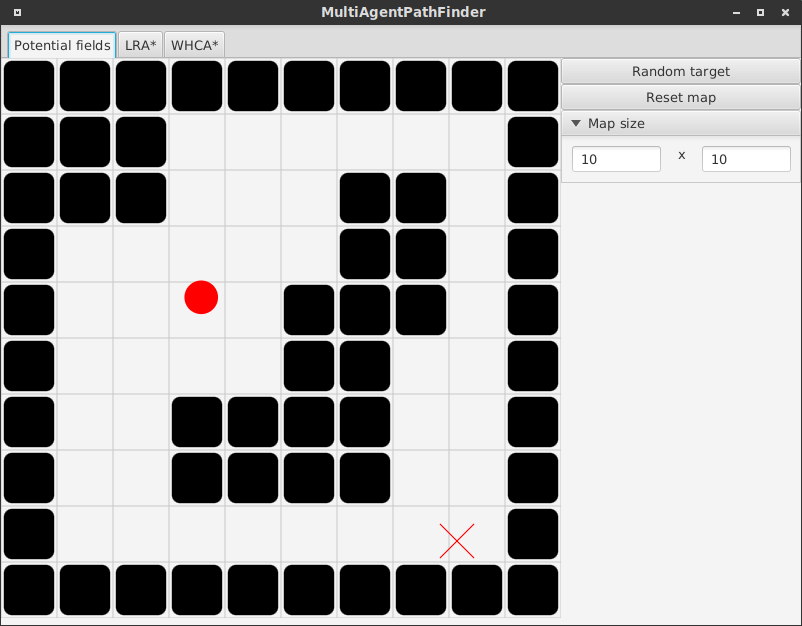
\includegraphics[width=0.8\columnwidth]{img/robopath/ui-fields}
	\caption{Zrzut ekranu aplikacji w trakcie wizualizacji metody pól potencjałowych.}
	\label{fig:robopath-ui-fields}
\end{figure}

\subsection{Local-Repair A*}

\begin{figure}
	\centering
	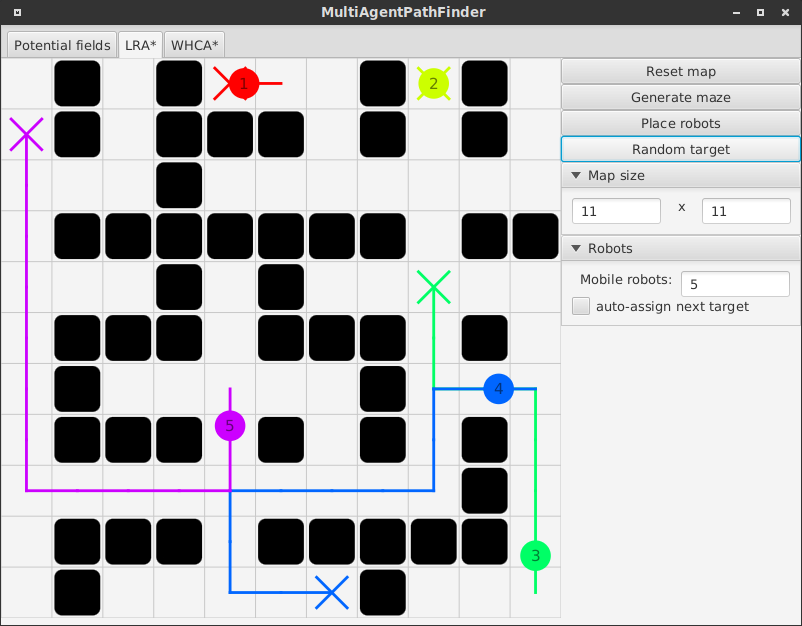
\includegraphics[width=0.8\columnwidth]{img/robopath/ui-lra}
	\caption{Zrzut ekranu aplikacji w trakcie wizualizacji metody Local-Repair A*.}
	\label{fig:robopath-ui-lra}
\end{figure}

\subsection{Windowed Hierarchical Cooperative A*}

\begin{figure}
	\centering
	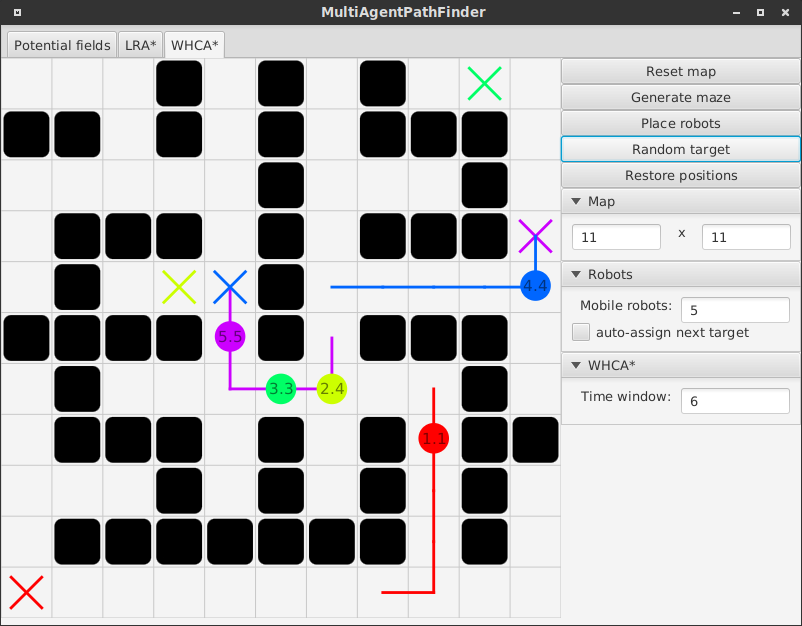
\includegraphics[width=0.8\columnwidth]{img/robopath/ui-whca}
	\caption{Zrzut ekranu aplikacji w trakcie wizualizacji metody Windowed Hierarchical Cooperative A*.}
	\label{fig:robopath-ui-whca}
\end{figure},


$TODO$ opis UI, zaznaczanie dróg, celów, płynne animacje, osobny wątek do UI
kółka to roboty, wyświetlanie ścieżek, celów
co robi każdy przycisk - instrukcja
3 zakładki: potential field, 
prawy klik
skalowalnosć, responsywność okna

\section{Wykorzystane technologie}
$TODO$ stack technologiczny, Wykorzystane technologie i narzędzia - opis technologii:
Java 8 - lambda, functional interfaces, streamy,
Java FX - FXML, Spring (core): IoC, DI; Spring Boot, testy jednostkowe jUnit, git, IntelliJ Ultimate, Maven, Linux, logback, Guava - joiner

uruchomienie aplikacji z kodów źródłowych : mvn spring-boot:run

\section{Testy}
$TODO$ TDD - Test driven development, testy jednostkowe do algorytmów pathfinding

\section{Struktura aplikacji}
$TODO$ lista beanów / serwisów, struktura widok, prezenter, kontroler; osobny wątek w tle do obliczeń + synchronizacja, wątek UI - zapewnienie REal-time, prawie MVP


\section{Screeny}
$TODO$ screeny

\section{Zaimplementowane metody}
$TODO$ potential fields, A*, LRA*, WHCA*

\section{featurey}
ustawianie random seeda
ponowne wykonanie symulacji - te same warunki
przełaczanie między metodami na zakładkach ?
wykonanie symulacji w pojedynczych krokach
resizable window - responsive
heuristic cache
działania na wektorach, immutable vector

\section{Ograniczenia}
$TODO$ nałożone uproszczenia: ruch skośny trwa tyle samo, czas dyskretny, brak czasu na obrót

$TODO$ publikacja na GitHub, licencja MIT, filmiki na YT